Six sizes are measured on the dual-socket AMD EPYC 7543 Oracle node (128 logical CPUs) with two threads and an exclusive campaign compute lock. Fresh processes time the prepared energy, energy plus total gradient, energy plus gradient and analytic Hessian, and both-parent all-root singlet TDA on corrected GFN2 orbitals. Three repeats are retained for nitroxyl, acetaldehyde and acetone; a closing budget fixed before larger-case measurements uses one for furan, cyclopentadiene and phthalimide. Model loading and converged-ground setup are outside the property timer; peak RSS covers the whole process. The first three cases use one CSF per parent and the last three two, so this is a practical size/rank benchmark. After exact nuclear-response acceleration, every affected gradient and Hessian timing is remeasured. Unaffected energy-only and TDA measurements are retained, with their execution hashes. External server load and single-repeat large-case variability limit fine timing comparisons.

Across all six measured sizes, the retained prepared OO energy costs more than the complete both-parent TDA evaluation: 0.286--11.478~s versus 0.014--8.731~s. Thus no energy-only speed advantage is observed, even though TDA produces more roots. The intended contribution is the stationary energy surface and its complete analytic nuclear response.

With the contracted response, furan takes 0.851~s for energy plus gradient and 5.104~s including its analytic Hessian; cyclopentadiene takes 1.042 and 7.083~s. Their previous Hessian times were 104.156 and 251.653~s, giving measured reductions by factors of 20.4 and 35.5. Phthalimide now completes energy, gradient and the full $48\times48$ analytic Hessian in 42.224~s, compared with the previous right-censored time of at least 600~s: a reduction exceeding 14.2. Its energy-plus-gradient call takes 9.292~s. The maximum whole-process RSS in the updated benchmark is 1.07~GiB; the earlier phthalimide gradient process reached 9.26~GiB. All six Hessians are completed. The 72-row ledger contains 48 measured completed evaluations and 24 prespecified omitted repeats; earlier measurements and the censored attempt remain archived.

\begin{figure}[!htbp]
\centering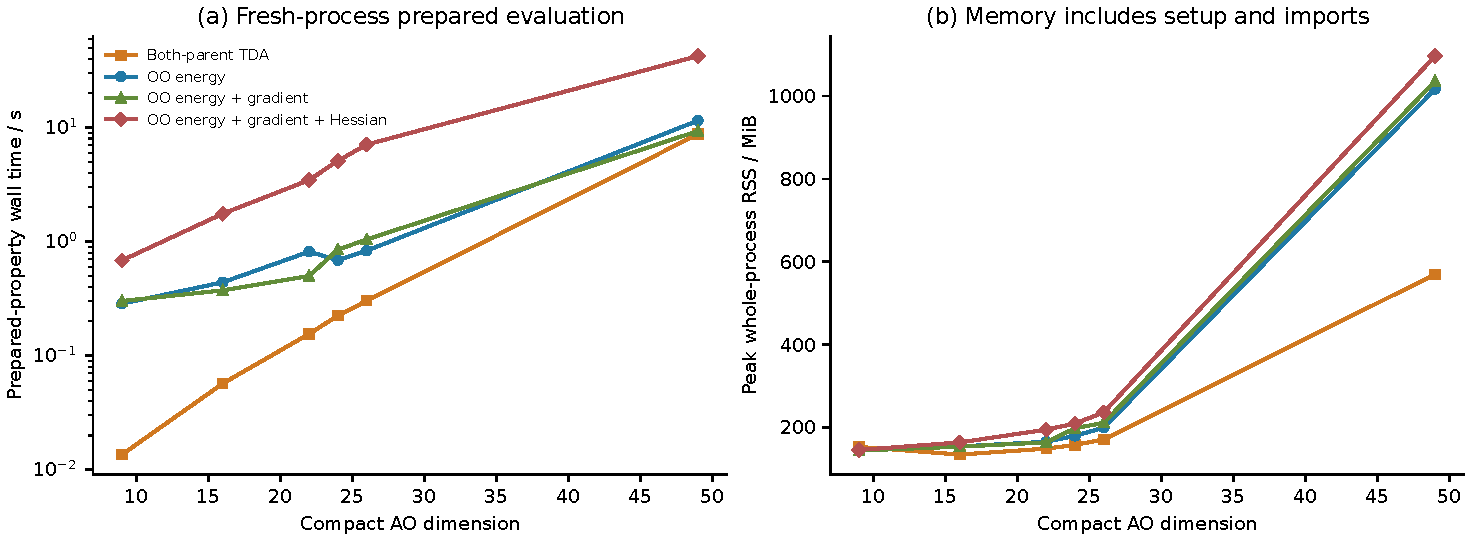
\includegraphics[width=\linewidth]{figures/final_cost_scaling.pdf}
\caption{Prepared-property wall time and whole-process peak RSS after analytic nuclear-response acceleration. Unaffected energy-only and TDA measurements are retained; gradients and Hessians are remeasured. TDA obtains all roots for both parents, whereas OO targets one state. The table records repetitions and ranks. Electronic work from this campaign does not overlap timings; external Oracle load is uncontrolled.}\label{fig:finalcost}
\end{figure}

Preparation is audited rather than assigned zero cost. For the fresh molecular cohort, DFT ground calculations take 0.51--38.13~s, recorded reference-TDA stages 0.88--73.36~s per symmetry, and executed full-response calibrations 1.52--77.17~s. Reference TDA supplies state identity and the active-rank rule: the current preparation therefore requires excited-reference transitions as well as ground-state DFT energies. These stage measurements are from a different cohort and are not missing preparation totals for the six timing molecules. Historical complete cold-preparation totals are unavailable. Consequently, the prepared costs quantify the derivative workload but do not establish an end-to-end advantage over TDA or a fully semiempirical reference preparation.
